% Options for packages loaded elsewhere
\PassOptionsToPackage{unicode}{hyperref}
\PassOptionsToPackage{hyphens}{url}
%
\documentclass[
]{book}
\usepackage{amsmath,amssymb}
\usepackage{lmodern}
\usepackage{ifxetex,ifluatex}
\ifnum 0\ifxetex 1\fi\ifluatex 1\fi=0 % if pdftex
  \usepackage[T1]{fontenc}
  \usepackage[utf8]{inputenc}
  \usepackage{textcomp} % provide euro and other symbols
\else % if luatex or xetex
  \usepackage{unicode-math}
  \defaultfontfeatures{Scale=MatchLowercase}
  \defaultfontfeatures[\rmfamily]{Ligatures=TeX,Scale=1}
\fi
% Use upquote if available, for straight quotes in verbatim environments
\IfFileExists{upquote.sty}{\usepackage{upquote}}{}
\IfFileExists{microtype.sty}{% use microtype if available
  \usepackage[]{microtype}
  \UseMicrotypeSet[protrusion]{basicmath} % disable protrusion for tt fonts
}{}
\makeatletter
\@ifundefined{KOMAClassName}{% if non-KOMA class
  \IfFileExists{parskip.sty}{%
    \usepackage{parskip}
  }{% else
    \setlength{\parindent}{0pt}
    \setlength{\parskip}{6pt plus 2pt minus 1pt}}
}{% if KOMA class
  \KOMAoptions{parskip=half}}
\makeatother
\usepackage{xcolor}
\IfFileExists{xurl.sty}{\usepackage{xurl}}{} % add URL line breaks if available
\IfFileExists{bookmark.sty}{\usepackage{bookmark}}{\usepackage{hyperref}}
\hypersetup{
  pdftitle={Evaluating Informative Hypotheses With Equality and Inequality Constraint: The Bayes Factor Encompassing Prior Approach},
  pdfauthor={Claudio Zandonella Callegher, Tatiana Marci, Pietro De Carli, and Gianmarco Altoè},
  hidelinks,
  pdfcreator={LaTeX via pandoc}}
\urlstyle{same} % disable monospaced font for URLs
\usepackage{longtable,booktabs,array}
\usepackage{calc} % for calculating minipage widths
% Correct order of tables after \paragraph or \subparagraph
\usepackage{etoolbox}
\makeatletter
\patchcmd\longtable{\par}{\if@noskipsec\mbox{}\fi\par}{}{}
\makeatother
% Allow footnotes in longtable head/foot
\IfFileExists{footnotehyper.sty}{\usepackage{footnotehyper}}{\usepackage{footnote}}
\makesavenoteenv{longtable}
\usepackage{graphicx}
\makeatletter
\def\maxwidth{\ifdim\Gin@nat@width>\linewidth\linewidth\else\Gin@nat@width\fi}
\def\maxheight{\ifdim\Gin@nat@height>\textheight\textheight\else\Gin@nat@height\fi}
\makeatother
% Scale images if necessary, so that they will not overflow the page
% margins by default, and it is still possible to overwrite the defaults
% using explicit options in \includegraphics[width, height, ...]{}
\setkeys{Gin}{width=\maxwidth,height=\maxheight,keepaspectratio}
% Set default figure placement to htbp
\makeatletter
\def\fps@figure{htbp}
\makeatother
\setlength{\emergencystretch}{3em} % prevent overfull lines
\providecommand{\tightlist}{%
  \setlength{\itemsep}{0pt}\setlength{\parskip}{0pt}}
\setcounter{secnumdepth}{5}
\usepackage{booktabs}
\usepackage{amsthm}
\makeatletter
\def\thm@space@setup{%
  \thm@preskip=8pt plus 2pt minus 4pt
  \thm@postskip=\thm@preskip
}
\makeatother


%----    define infoboxes    ----%
\usepackage{tcolorbox}
\usepackage{xcolor}

% colors
\definecolor{background}{HTML}{fcfcfc}
\definecolor{tip-text}{HTML}{e7b002}
\definecolor{tip-line}{HTML}{fdce38}
\definecolor{warning-text}{HTML}{b06336}
\definecolor{warning-line}{HTML}{c97d50}
\definecolor{deffun-text}{HTML}{0b797e}
\definecolor{deffun-line}{HTML}{6CC2C9}
\definecolor{design-text}{HTML}{7c972e}
\definecolor{design-line}{HTML}{a7c84a}
\definecolor{trick-text}{HTML}{8c3031}
\definecolor{trick-line}{HTML}{A3595A}

\newtcolorbox{mybox}[1][black]{
  colback=background,
  coltext=black,
  colframe=#1,
  boxsep=5pt,
  arc=4pt}

% tip
\newenvironment{tip}[1][Title]
  {
  \setlength{\fboxsep}{1em}
  \begin{mybox}[tip-line]
    \raisebox{-.2\height}{\includegraphics[height=.6cm]{images/lightbulb.png}} \large \textcolor{tip-text}{Tip-Box: #1}
    \vspace{1em}
    }
    {
  \end{mybox}
  }

% warning
\newenvironment{warning}[1][Title]
  {
  \setlength{\fboxsep}{1em}
  \begin{mybox}[warning-line]
    \raisebox{-.2\height}{\includegraphics[height=.6cm]{images/gotcha.png}} \large \textcolor{warning-text}{Warning-Box: #1}
    \vspace{1em}
    }
    {
  \end{mybox}
  }

% deffun
\newenvironment{deffun}[1][Title]
  {
  \setlength{\fboxsep}{1em}
  \begin{mybox}[deffun-line]
    \raisebox{-.2\height}{\includegraphics[height=.6cm]{images/gears.png}} \large \textcolor{deffun-text}{Definition-Box: #1}
    \vspace{1em}
    }
    {
  \end{mybox}
  }

% design
\newenvironment{design}[1][Title]
  {
  \setlength{\fboxsep}{1em}
  \begin{mybox}[design-line]
    \raisebox{-.2\height}{\includegraphics[height=.6cm]{images/design.png}} \large \textcolor{design-text}{Design-Box: #1}
    \vspace{1em}
    }
    {
  \end{mybox}
  }

% trick
\newenvironment{trick}[1][Title]
  {
  \setlength{\fboxsep}{1em}
  \begin{mybox}[trick-line]
    \raisebox{-.2\height}{\includegraphics[height=.6cm]{images/hat.png}} \large \textcolor{trick-text}{Trick-Box: #1}
    \vspace{1em}
    }
    {
  \end{mybox}
  }


\usepackage{titlepic}
\titlepic{
\includegraphics[width=\textwidth]{images/logo_psicostat.pdf}}
\ifluatex
  \usepackage{selnolig}  % disable illegal ligatures
\fi
\usepackage[]{natbib}
\bibliographystyle{plainnat}

\title{Evaluating Informative Hypotheses With Equality and Inequality Constraint: The Bayes Factor Encompassing Prior Approach}
\usepackage{etoolbox}
\makeatletter
\providecommand{\subtitle}[1]{% add subtitle to \maketitle
  \apptocmd{\@title}{\par {\large #1 \par}}{}{}
}
\makeatother
\subtitle{Supplemental Material}
\author{Claudio Zandonella Callegher, Tatiana Marci, Pietro De Carli, and Gianmarco Altoè}
\date{2021-09-14}

\begin{document}
\maketitle

{
\setcounter{tocdepth}{1}
\tableofcontents
}
\begin{verbatim}
## i Loading Attachment
\end{verbatim}

\hypertarget{prerequisites}{%
\chapter*{Prerequisites}\label{prerequisites}}
\addcontentsline{toc}{chapter}{Prerequisites}

trial

\hypertarget{intro}{%
\chapter{Introduction}\label{intro}}

trial code

\begin{verbatim}
##   ID ID_class externalizing_sum internalizing_sum gender age_year Avm      Avp
## 1 25        2                16                 7      F     8.42 1.0 1.000000
## 2 27        2                 3                 3      F     9.00 2.0 2.166667
## 3 29        2                 5                 5      M     9.00 3.5 2.200000
## 4 30        2                11                11      M     8.92 1.6 2.666667
## 5 31        2                 0                 1      F     9.00 2.0 2.800000
## 6 32        2                 4                12      F     8.92 3.0 2.833333
##        av_m      av_p     Anxm     Anxp     anx_m     anx_p  mother   father
## 1 1.0000000 1.0000000 1.000000 1.000000 0.8333333 1.0000000  Secure   Secure
## 2 1.0000000 1.0000000 1.000000 1.000000 1.0000000 1.0000000 Anxious   Secure
## 3 1.0000000 0.8333333 1.500000 2.400000 1.0000000 0.8333333 Fearful  Anxious
## 4 0.8333333 1.0000000 1.600000 1.666667 0.8333333 1.0000000 Anxious Avoidant
## 5 1.0000000 0.8333333 1.833333 1.333333 1.0000000 1.0000000 Anxious Avoidant
## 6 1.0000000 1.0000000 3.200000 2.833333 0.8333333 1.0000000 Anxious  Fearful
##            interaction
## 1    M_Secure_F_Secure
## 2   M_Anxious_F_Secure
## 3  M_Fearful_F_Anxious
## 4 M_Anxious_F_Avoidant
## 5 M_Anxious_F_Avoidant
## 6  M_Anxious_F_Fearful
\end{verbatim}

plot trial

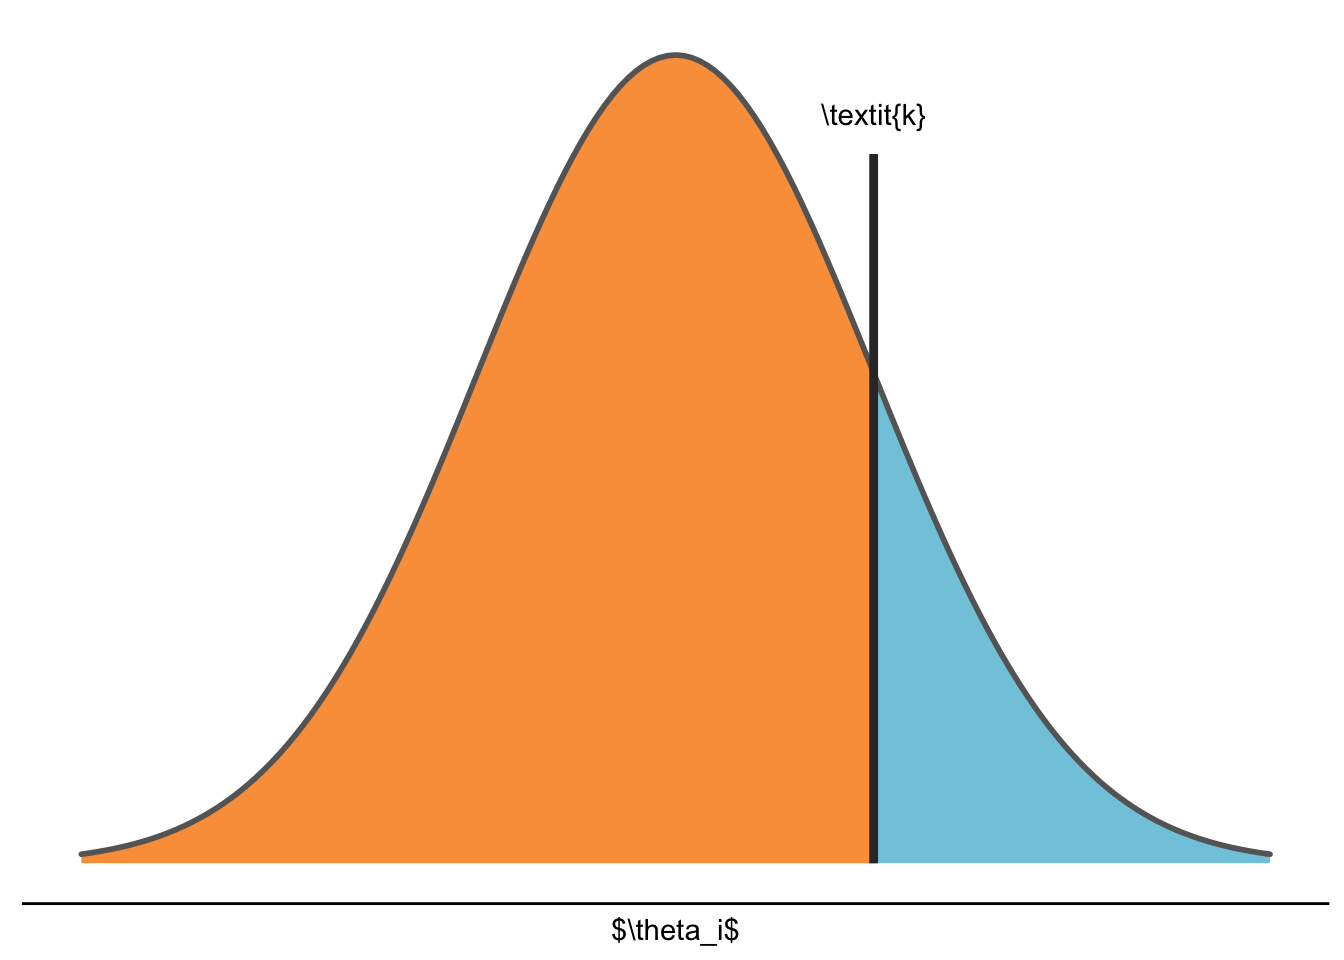
\includegraphics{attachment-bayes-factor_files/figure-latex/unnamed-chunk-3-1.pdf}

table trial

\begin{table}[!h]

\caption{\label{tab:unnamed-chunk-4}Attachment styles frequencies ($n_{subj} = 847$).}
\centering
\begin{tabular}[t]{rccccc}
\toprule
\multicolumn{1}{c}{\textbf{ }} & \multicolumn{4}{c}{\textbf{Father Attachment}} & \multicolumn{1}{c}{\textbf{ }} \\
\cmidrule(l{3pt}r{3pt}){2-5}
\textbf{Mother Attachemnt} & \textbf{Secure} & \textbf{Anxious} & \textbf{Avoidant} & \textbf{Fearful} & \textbf{Total}\\
\midrule
Secure & 125 & 49 & 49 & 8 & 231\\
Anxious & 51 & 100 & 98 & 37 & 286\\
Avoidant & 25 & 67 & 126 & 12 & 230\\
Fearful & 5 & 14 & 38 & 43 & 100\\
Total & 206 & 230 & 311 & 100 & 847\\
\bottomrule
\end{tabular}
\end{table}

trial citation

\citep{guApproximatedAdjustedFractional2018}

troppe cit \citep{mcelreathStatisticalRethinkingBayesian2020}

  \bibliography{../Biblio-attachment.bib}

\end{document}
